%%%%%%%%%%%%%%%%%%%%%%%%%%%%%%%%%%%%%%%%%%%%%%
%% Compile: XeLaTeX BibTeX XeLaTeX XeLaTeX
%% Loesung-Handout: Antonio Machicao y Priemer
%% Course: GK Linguistik
%%%%%%%%%%%%%%%%%%%%%%%%%%%%%%%%%%%%%%%%%%%%%%

%\documentclass[a4paper,10pt, bibtotoc]{beamer}
\documentclass[10pt,handout]{beamer}

%%%%%%%%%%%%%%%%%%%%%%%%
%%     PACKAGES      
%%%%%%%%%%%%%%%%%%%%%%%%

%%%%%%%%%%%%%%%%%%%%%%%%
%%     PACKAGES       %%
%%%%%%%%%%%%%%%%%%%%%%%%



%\usepackage[utf8]{inputenc}
%\usepackage[vietnamese, english,ngerman]{babel}   % seems incompatible with german.sty
%\usepackage[T3,T1]{fontenc} breaks xelatex
\usepackage{lmodern}

\usepackage{amsmath}
\usepackage{amsfonts}
\usepackage{amssymb}
%% MnSymbol: Mathematische Klammern und Symbole (Inkompatibel mit ams-Packages!)
%% Bedeutungs- und Graphemklammern: $\lsem$ Tisch $\rsem$ $\langle TEXT \rangle$ $\llangle$ TEXT $\rrangle$ 
\usepackage{MnSymbol}
%% ulem: Strike out
\usepackage[normalem]{ulem}  

%% Special Spaces (s. Commands)
\usepackage{xspace}				
\usepackage{setspace}
%	\onehalfspacing

%% mdwlist: Special lists
\usepackage{mdwlist}	

\usepackage[noenc,safe]{tipa}

% maybe define \textipa to use \originalTeX to avoid problems with `"'.
%
%	\ex \textipa{\originalTeX [pa.pa."g\t{aI}]}

%

\usepackage{etex}		%For Forest bug

%
%\usepackage{jambox}
%


%\usepackage{forest-v105}
%\usepackage{modified-langsci-forest-setup}

\usepackage{xeCJK}
\setCJKmainfont{SimSun}


%\usepackage{natbib}
%\setcitestyle{notesep={:~}}




% for toggles
\usepackage{etex}



% Fraktur!
\usepackage{yfonts}

\usepackage{url}

% für UDOP
\usepackage{adjustbox}


%% huberlin: Style sheet
%\usepackage{huberlin}
\usepackage{hu-beamer-includes-pdflatex}
\huberlinlogon{0.86cm}


%% Last Packages
%\usepackage{hyperref}	%URLs
%\usepackage{gb4e}		%Linguistic examples

% sorry this was incompatible with gb4e and had to go.
%\usepackage{linguex-cgloss}	%Linguistic examples (patched version that works with jambox

\usepackage{multirow}  %Mehrere Zeilen in einer Tabelle
%\usepackage{array}
\usepackage{marginnote}	%Notizen




%%%%%%%%%%%%%%%%%%%%%%%%%%%%%%%%%%%%%%%%%%%%%%%%%%%%
%%%          Commands                            %%%
%%%%%%%%%%%%%%%%%%%%%%%%%%%%%%%%%%%%%%%%%%%%%%%%%%%%

%%%%%%%%%%%%%%%%%%%%%%%%%%%%%%%%
% German quotation marks:
\newcommand{\gqq}[1]{\glqq{}#1\grqq{}}		%double
\newcommand{\gq}[1]{\glq{}#1\grq{}}			%simple


%%%%%%%%%%%%%%%%%%%%%%%%%%%%%%%%
% Abbreviations in German
% package needed: xspace
% Short space in German abbreviations: \,	
\newcommand{\idR}{\mbox{i.\,d.\,R.}\xspace}
\newcommand{\su}{\mbox{s.\,u.}\xspace}
%\newcommand{\ua}{\mbox{u.\,a.}\xspace}       % in abbrev
%\newcommand{\zB}{\mbox{z.\,B.}\xspace}       % in abbrev
%\newcommand{\s}{s.~}
%not possibel: \dh --> d.\,h.


%%%%%%%%%%%%%%%%%%%%%%%%%%%%%%%%
%Abbreviations in English
\newcommand{\ao}{a.o.\ }	% among others
\newcommand{\cf}[1]{(cf.~#1)}	% confer = compare
\renewcommand{\ia}{i.a.}	% inter alia = among others
\newcommand{\ie}{i.e.~}	% id est = that is
\newcommand{\fe}{e.g.~}	% exempli gratia = for example
%not possible: \eg --> e.g.~
\newcommand{\vs}{vs.\ }	% versus
\newcommand{\wrt}{w.r.t.\ }	% with respect to


%%%%%%%%%%%%%%%%%%%%%%%%%%%%%%%%
% Dash:
\newcommand{\gs}[1]{--\,#1\,--}


%%%%%%%%%%%%%%%%%%%%%%%%%%%%%%%%
% Rightarrow with and without space
\def\ra{\ensuremath\rightarrow}			%without space
\def\ras{\ensuremath\rightarrow\ }		%with space


%%%%%%%%%%%%%%%%%%%%%%%%%%%%%%%%
%% X-bar notation

%% Notation with primes (not emphasized): \xbar{X}
\newcommand{\MyPxbar}[1]{#1$^{\prime}$}
\newcommand{\xxbar}[1]{#1$^{\prime\prime}$}
\newcommand{\xxxbar}[1]{#1$^{\prime\prime\prime}$}

%% Notation with primes (emphasized): \exbar{X}
\newcommand{\exbar}[1]{\emph{#1}$^{\prime}$}
\newcommand{\exxbar}[1]{\emph{#1}$^{\prime\prime}$}
\newcommand{\exxxbar}[1]{\emph{#1}$^{\prime\prime\prime}$}

% Notation with zero and max (not emphasized): \xbar{X}
\newcommand{\zerobar}[1]{#1$^{0}$}
\newcommand{\maxbar}[1]{#1$^{\textsc{max}}$}

% Notation with zero and max (emphasized): \xbar{X}
\newcommand{\ezerobar}[1]{\emph{#1}$^{0}$}
\newcommand{\emaxbar}[1]{\emph{#1}$^{\textsc{max}}$}

%% Notation with bars (already implemented in gb4e):
% \obar{X}, \ibar{X}, \iibar{X}, \mbar{X} %Problems with \mbar!
%
%% Without gb4e:
\newcommand{\overbar}[1]{\mkern 1.5mu\overline{\mkern-1.5mu#1\mkern-1.5mu}\mkern 1.5mu}
%
%% OR:
\newcommand{\MyPibar}[1]{$\overline{\textrm{#1}}$}
\newcommand{\MyPiibar}[1]{$\overline{\overline{\textrm{#1}}}$}
%% (emphasized):
\newcommand{\eibar}[1]{$\overline{#1}$}
\newcommand{\eiibar}[1]{\overline{$\overline{#1}}$}

%%%%%%%%%%%%%%%%%%%%%%%%%%%%%%%%
%% Subscript & Superscript: no italics
\newcommand{\MyPdown}[1]{$_{\textrm{#1}}$}
\newcommand{\MyPup}[1]{$^{\textrm{#1}}$}


%%%%%%%%%%%%%%%%%%%%%%%%%%%%%%%%
% Objekt language marking:
%\newcommand{\obj}[1]{\glqq{}#1\grqq{}}	%German double quotes
%\newcommand{\obj}[1]{``#1''}			%English double quotes
\newcommand{\MyPobj}[1]{\emph{#1}}		%Emphasising


%%%%%%%%%%%%%%%%%%%%%%%%%%%%%%%%
%% Semantic types (<e,t>), features, variables and graphemes in angled brackets 

%%% types and variables, in math mode: angled brackets + italics + no space
%\newcommand{\type}[1]{$<#1>$}

%%% OR more correctly: 
%%% types and variables, in math mode: chevrons! + italics + no space
\newcommand{\MyPtype}[1]{$\langle #1 \rangle$}

%%% features and graphemes, in math mode: chevrons! + italics + no space
\newcommand{\abe}[1]{$\langle #1 \rangle$}


%%% features and graphemes, in math mode: chevrons! + no italics + space
\newcommand{\ab}[1]{$\langle$#1$\rangle$}  %%same as \abu  
\newcommand{\abu}[1]{$\langle$#1$\rangle$} %%Umlaute

%%% Notizen
\renewcommand{\marginfont}{\singlespacing}
\renewcommand{\marginfont}{\footnotesize}
\renewcommand{\marginfont}{\color{black}}

\newcommand{\myp}[1]{%
	\marginnote{%
		\begin{spacing}{1}
			\vspace{-\baselineskip}%
			\color{red}\footnotesize#1
		\end{spacing}
	}
}
%%%%%%%%%%%%%%%%%%%%%%%%%%%%%%%%
%% Outputbox
\newcommand{\outputbox}[1]{\noindent\fbox{\parbox[t][][t]{0.98\linewidth}{#1}}\vspace{0.5em}}

%%%%%%%%%%%%%%%%%%%%%%%%%%%%%%%%
%% (Syntactic) Trees
% package needed: forest
%
%% Setting for simple trees
\forestset{
	MyP edges/.style={for tree={parent anchor=south, child anchor=north}}
}

%% this is taken from langsci-setup file
%% Setting for complex trees
%% \forestset{
%% 	sn edges/.style={for tree={parent anchor=south, child anchor=north,align=center}}, 
%% background tree/.style={for tree={text opacity=0.2,draw opacity=0.2,edge={draw opacity=0.2}}}
%% }

\newcommand\HideWd[1]{%
	\makebox[0pt]{#1}%
}


%%%%%%%%%%%%%%%%%%%%%%%%%%%%%%%%%%%%%%%%%%%%%%%%%%%%
%%%          Useful commands                     %%%
%%%%%%%%%%%%%%%%%%%%%%%%%%%%%%%%%%%%%%%%%%%%%%%%%%%%

%%%%%%%%%%%%%%%%%%%%%
%% FOR ITEMS:
%\begin{itemize}
%  \item<2-> from point 2
%  \item<3-> from point 3 
%  \item<4-> from point 4 
%\end{itemize}
%
% or: \onslide<2->
% or: \pause

%%%%%%%%%%%%%%%%%%%%%
%% VERTICAL SPACE:
% \vspace{.5cm}
% \vfill

%%%%%%%%%%%%%%%%%%%%%
% RED MARKING OF TEXT:
%\alert{bis spätestens Mittwoch, 18 Uhr}

%%%%%%%%%%%%%%%%%%%%%
%% RESCALE BIG TABLES:
%\scalebox{0.8}{
%For Big Tables
%}

%%%%%%%%%%%%%%%%%%%%%
%% BLOCKS:
%\begin{alertblock}{Title}
%Text
%\end{alertblock}
%
%\begin{block}{Title}
%Text
%\end{block}
%
%\begin{exampleblock}{Title}
%Text
%\end{exampleblock}


\newtoggle{uebung}
\newtoggle{loesung}
\newtoggle{toc}

% The toc is not needed on Handouts. Safe trees.
\mode<handout>{
\togglefalse{toc}
}

\newtoggle{hpsgvorlesung}\togglefalse{hpsgvorlesung}
\newtoggle{syntaxvorlesungen}\togglefalse{syntaxvorlesungen}

%\includecomment{psgbegriffe}
%\excludecomment{konstituentenprobleme}
%\includecomment{konstituentenprobleme-hinweis}

\newtoggle{konstituentenprobleme}\togglefalse{konstituentenprobleme}
\newtoggle{konstituentenprobleme-hinweis}\toggletrue{konstituentenprobleme-hinweis}

%\includecomment{einfsprachwiss-include}
%\excludecomment{einfsprachwiss-exclude}
\newtoggle{einfsprachwiss-include}\toggletrue{einfsprachwiss-include}
\newtoggle{einfsprachwiss-exclude}\togglefalse{einfsprachwiss-exclude}

\newtoggle{psgbegriffe}\toggletrue{psgbegriffe}

\newtoggle{gb-intro}\togglefalse{gb-intro}



%%%%%%%%%%%%%%%%%%%%%%%%%%%%%%%%%%%%%%%%%%%%%%%%%%%%
%%%             Preamble's End                   
%%%%%%%%%%%%%%%%%%%%%%%%%%%%%%%%%%%%%%%%%%%%%%%%%%%% 

\begin{document}
	

%%%% ue-loesung
%%%% true: Übung & Lösungen (slides) / false: nur Übung (handout)
%	\toggletrue{ue-loesung}

%%%% ha-loesung
%%%% true: Hausaufgabe & Lösungen (slides) / false: nur Hausaufgabe (handout)
%	\toggletrue{ha-loesung}

%%%% toc
%%%% true: TOC am Anfang von Slides / false: keine TOC am Anfang von Slides
\toggletrue{toc}

%%%% sectoc
%%%% true: TOC für Sections / false: keine TOC für Sections (StM handout)
%	\toggletrue{sectoc}

%%%% gliederung
%%%% true: Gliederung für Sections / false: keine Gliederung für Sections
%	\toggletrue{gliederung}


%%%%%%%%%%%%%%%%%%%%%%%%%%%%%%%%%%%%%%%%%%%%%%%%%%%%
%%%             Metadata                         
%%%%%%%%%%%%%%%%%%%%%%%%%%%%%%%%%%%%%%%%%%%%%%%%%%%%      

\title{Grundkurs Linguistik}

\subtitle{Lösungen -- Phonologie III}

\author[A. Machicao y Priemer]{
	{\small Antonio Machicao y Priemer}
	\\
	{\footnotesize \url{http://www.linguistik.hu-berlin.de/staff/amyp}}
	%	\\
	%	\href{mailto:mapriema@hu-berlin.de}{mapriema@hu-berlin.de}}
}

\institute{Institut für deutsche Sprache und Linguistik}


% bitte lassen, sonst kann man nicht sehen, von wann die PDF-Datei ist.
%\date{ }

%\publishers{\textbf{6. linguistischer Methodenworkshop \\ Humboldt-Universität zu Berlin}}

%\hyphenation{nobreak}


%%%%%%%%%%%%%%%%%%%%%%%%%%%%%%%%%%%%%%%%%%%%%%%%%%%%
%%%             Preamble's End                  
%%%%%%%%%%%%%%%%%%%%%%%%%%%%%%%%%%%%%%%%%%%%%%%%%%%%      


%%%%%%%%%%%%%%%%%%%%%%%%%      
\huberlintitlepage[22pt]
\iftoggle{toc}{
	\frame{
		\begin{multicols}{2}
		\frametitle{Inhaltsverzeichnis}
		\tableofcontents
		%[pausesections]
	\columnbreak
		\textcolor{white}{
			\ea \label{ex:fabrik}
			\ex\label{ex:ebbe}
			\ex\label{ex:otling}
			\ex\label{ex:blumen}
			\ex\label{ex:03cHA1}
				\ea\label{ex:03cHA1a}
				\ex\label{ex:03cHA1b}
				\ex\label{ex:03cHA1c}
				\z
			\ex\label{ex:03cHA2}
			\ex\label{ex:03cHA3}
			\z
		}
		\end{multicols}
	}
}


%%%%%%%%%%%%%%%%%%%%%%%%%%%%%%%%%%%
%%%%%%%%%%%%%%%%%%%%%%%%%%%%%%%%%%%
\section{Übungen}

%%%%%%%%%%%%%%%%%%%%%%%%%%%%%%%%%%
%% UE 1 - 03c Phonologie
%%%%%%%%%%%%%%%%%%%%%%%%%%%%%%%%%%

\begin{frame}
\frametitle{Übung -- Lösung}

\begin{minipage}{.45\textwidth}
\centering
\scalebox{.75}{	
\begin{forest} MyP edges, [,phantom
[$\sigma$
[O	[x, tier=word [\textipa{S}]
]
[x, tier=word [\textipa{p}]
]
[x, tier=word[\textipa{\textscr}]
]
]
[R
[N	[x, tier=word [\textipa{E}]
]
]
[K, name=K	[x,name=x  [\textipa{\c{c}}]
]
]
]  
]
[$\sigma$
[O, name=O]
[R
[N	[x[\textipa{@}]
]
]
[K	[x[\textipa{n}]
]
]
]
]
]
\draw[black] (O.south)--(x.north);
\end{forest}
}
\end{minipage}
\pause
%
\begin{minipage}{.05\textwidth}
\hfill
\end{minipage}
%
\begin{minipage}{.45\textwidth}
%%%%%%%%%%%%%%%
%%% Forestset Syllables

\newbox\foreststrutbox
\setbox\foreststrutbox=\hbox to 0pt{\phantom{\forestOve{standard node}{content}}}
\def\foreststrut{\copy\foreststrutbox}
\forestset{
GP1/.style 2 args={
for n={1}{baseline},
s sep=0pt, l sep=0pt,
for descendants={
l sep=0pt, l={#1},
anchor=base,calign=first,child anchor=north,
inner xsep=1pt,inner ysep=2pt,outer sep=0pt,s sep=0pt,
},
delay={
if content={}{phantom}{for children={no edge}},
for tree={
if content={O}{tier=OR}{},
if content={R}{tier=OR}{},
if content={N}{tier=N}{},
if content={x}{
tier=x,content={$\times$},outer xsep={#2},
for tree={calign=center},
for descendants={content format={\foreststrut\forestoption{content}}},
before drawing tree={outer xsep=0pt,delay={typeset node}},
s sep=4pt
}{},
},
},
before drawing tree={where content={}{parent anchor=center,child anchor=center}{}},
},
GP1/.default={5ex}{8.0pt},
associate/.style={%
tikz+={\draw(!)--(!#1);}},
spread/.style={
before drawing tree={tikz+={\draw[dotted](!)--(!#1);}}},
govern/.style={
before drawing tree={tikz+={\draw[->](!)--(!#1);}}},
p-govern/.style={
before drawing tree={tikz+={\draw[->](.north) to[out=150,in=30] (!#1.north);}}},
no p-govern/.style={
before drawing tree={tikz+={\draw[->,loosely dashed](.north) to[out=150,in=30] (!#1.north);}}},
encircle/.style={before drawing tree={circle,draw,inner sep=0pt}},
fen/.style={pin={[font=\footnotesize,inner sep=1pt,pin edge=<-]10:\textsc{Fen}}},
el/.style={content=\textsc{\textbf{##1}}},
head/.style={content=\textsc{\textbf{\underline{##1}}}},
llap/.style={
tikz+={%
\edef\forest@temp{\noexpand\node[\option{node options},
anchor=base east,at=(.base east)]}%
\forest@temp{#1\phantom{\option{environment}}};
}
},
rlap/.style={
tikz+={%
\edef\forest@temp{\noexpand\node[\option{node options},
anchor=base west,at=(.base west)]}%
\forest@temp{\phantom{\option{environment}}#1};
}
},
}
%%%%%%%%%%%%%

\centering
%\visible<3->
{\scalebox{.75}{\begin{forest} MyP edges, [,phantom
[$\sigma$
[O	[x, tier=word[\textipa{P}]
]
]
[R
[N
[x, tier=word[\textipa{o:}, name=o]
]
[x, name=x]
%    		{\draw[black] (.south)--++(-2.38em,-1.7ex);}
]
[K
[x[\textipa{p}]
]
[x[\textipa{s}]
]
[x[\textipa{t}]
]
]
]  
] ]
\draw[black](x.south)--(o.north);
\end{forest}}}
\end{minipage}
\pause
\begin{minipage}{.45\textwidth}
\begin{figure}
\centering
%		\visible<2->
{\scalebox{.75}{
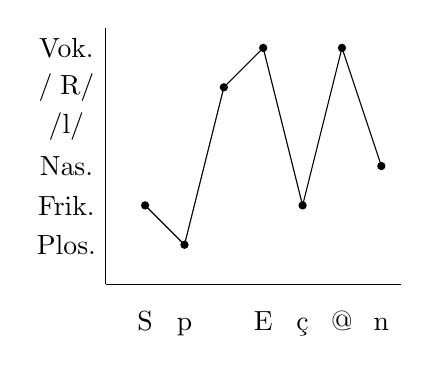
\begin{tikzpicture}[scale=0.5]
\draw[black] (-1,0) -- (6.5,0) ; % x axis
\draw[black] (-1,0) -- (-1,6.5); % y axis
\node at (-2,1) {Plos.};
\node at (-2,2) {Frik.};
\node at (-2,3) {Nas.};
\node at (-2,4) {\textipa{/l/}};
\node at (-2,5) {\textipa{/\;R/}};
\node at (-2,6) {Vok.};
\draw[black] (0,2) -- (1,1) -- (2,5) -- (3,6) -- (4,2) -- (5,6) -- (6,3);
\node at (0,-1) {\strut \textipa{S}};
\node at (1,-1) {\strut \textipa{p}};
\node at (2,-1) {\strut \textipa{\textscr}};
\node at (3,-1) {\strut \textipa{E}};
\node at (4,-1) {\strut \textipa{\c{c}}};
\node at (5,-1) {\strut \textipa{@}};
\node at (6,-1) {\strut \textipa{n}};
\fill (0,2) circle [radius=3pt];
\fill (1,1) circle [radius=3pt];
\fill (2,5) circle [radius=3pt];
\fill (3,6) circle [radius=3pt];
\fill (4,2) circle [radius=3pt];
\fill (5,6) circle [radius=3pt];
\fill (6,3) circle [radius=3pt];
\end{tikzpicture}}}
\end{figure}
\end{minipage}
\pause
\begin{minipage}{.05\textwidth}
\hfill
\end{minipage}
\begin{minipage}{.45\textwidth}
\begin{figure}
\centering
%\visible<4->
{\scalebox{.75}{
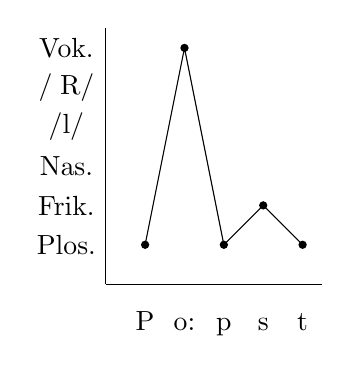
\begin{tikzpicture}[scale=0.5]
\draw[black] (-1,0) -- (4.5,0) ; % x axis
\draw[black] (-1,0) -- (-1,6.5); % y axis
\node at (-2,1) {Plos.};
\node at (-2,2) {Frik.};
\node at (-2,3) {Nas.};
\node at (-2,4) {\textipa{/l/}};
\node at (-2,5) {\textipa{/\;R/}};
\node at (-2,6) {Vok.};
\draw[black] (0,1) -- (1,6) -- (2,1) -- (3,2) -- (4,1);
\node at (0,-1) {\strut \textipa{P}};
\node at (1,-1) {\strut \textipa{o:}};
\node at (2,-1) {\strut \textipa{p}};
\node at (3,-1) {\strut \textipa{s}};
\node at (4,-1) {\strut \textipa{t}};
\fill (0,1) circle [radius=3pt];
\fill (1,6) circle [radius=3pt];
\fill (2,1) circle [radius=3pt];
\fill (3,2) circle [radius=3pt];
\fill (4,1) circle [radius=3pt];
\end{tikzpicture}}}
\end{figure}
\end{minipage}

\end{frame}
%%%%%%%%%%%%%%%%%%%%%%%%%%%%%%%%%

\begin{frame}
\frametitle{Übung -- Lösung}
%
\begin{minipage}{.3\textwidth}
\centering
\scalebox{.75}{\begin{forest} MyP edges, [,phantom
[$\sigma$
[O
[x, tier=word[\textipa{b}]]
[x, tier=word[\textipa{\textscr}]]
]
[R
[N	[x, tier=word[\textipa{a}]]
]
[K
[x[\textipa{n}]]
[x[\textipa{t}]]
]
]  
]
[$\sigma$
[O	[x, tier=word[\textipa{S}]]
]
[R	
[N	
[x[\textipa{U}]]
]
[K	
[x[\textipa{\t{ts}}]]
]
]
]]
\end{forest}}

\end{minipage}
\pause
%
\begin{minipage}{.02\textwidth}
\hfill
\end{minipage}
%
\begin{minipage}{.65\textwidth}
\centering
\scalebox{.75}{
\begin{forest}
MyP edges, [, phantom
[$ \sigma $
[O
[x, tier=word[\textipa{P}]]
]
[R
[N
[x, tier=word[\textipa{a}]]
]
[K
[x[\textipa{p}]]
]
]
]
[$ \sigma $
[O
[x, tier=word[\textipa{S}]]
[x, tier=word[\textipa{t}]]
]
[R
[N
[x[\textipa{a}]]
]
[K
[x[\textipa{n}]]
[x[\textipa{t}]]
[x[\textipa{s}]]
]
]
]
[$ \sigma $
[O
[x, tier=word[\textipa{h}]]
]
[R
[N
[x[\textipa{a}]]
]
[K
[x[\textipa{l}]]
]
]
]
[$ \sigma $
[O
[x, tier=word[t]]
]
[R	
[N
[x[\textipa{\textturna}]]
]
]
]]
\end{forest}}
\end{minipage}
\pause
\begin{minipage}{.3\textwidth}
\begin{figure}
\centering
\scalebox{.75}{
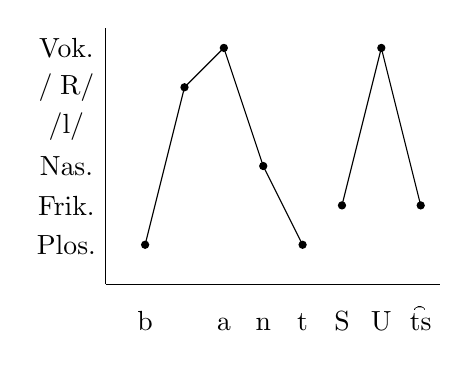
\begin{tikzpicture}[scale=0.5]
\draw[black] (-1,0) -- (7.5,0) ; % x axis
\draw[black] (-1,0) -- (-1,6.5); % y axis
\node at (-2,1) {Plos.};
\node at (-2,2) {Frik.};
\node at (-2,3) {Nas.};
\node at (-2,4) {\textipa{/l/}};
\node at (-2,5) {\textipa{/\;R/}};
\node at (-2,6) {Vok.};
\draw[black] (0,1) -- (1,5) -- (2,6) -- (3,3) -- (4,1);
\draw[black] (5,2) -- (6,6) -- (7,2);
\node at (0,-1) {\strut \textipa{b}};
\node at (1,-1) {\strut \textipa{\textscr}};
\node at (2,-1) {\strut \textipa{a}};
\node at (3,-1) {\strut \textipa{n}};
\node at (4,-1) {\strut \textipa{t}};
\node at (5,-1) {\strut \textipa{S}};
\node at (6,-1) {\strut \textipa{U}};
\node at (7,-1) {\strut \textipa{\t{ts}}};
\fill (0,1) circle [radius=3pt];
\fill (1,5) circle [radius=3pt];
\fill (2,6) circle [radius=3pt];
\fill (3,3) circle [radius=3pt];
\fill (4,1) circle [radius=3pt];
\fill (5,2) circle [radius=3pt];
\fill (6,6) circle [radius=3pt];
\fill (7,2) circle [radius=3pt];
\end{tikzpicture}}
\end{figure}
\end{minipage}
\pause
\begin{minipage}{.05\textwidth}
\hfill
\end{minipage}
\begin{minipage}{.6\textwidth}
\begin{figure}
\centering
\scalebox{.75}{
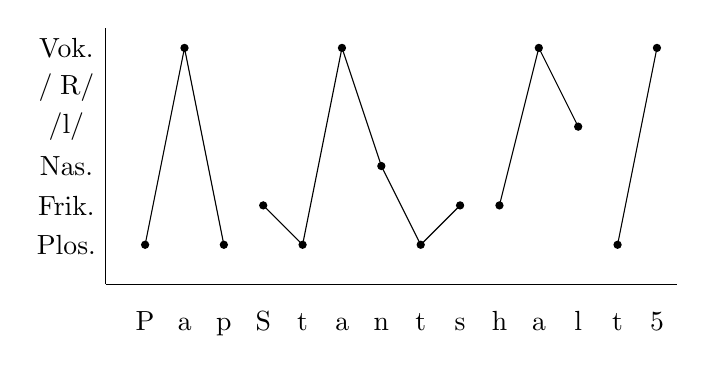
\begin{tikzpicture}[scale=0.5]
\draw[black] (-1,0) -- (13.5,0) ; % x axis
\draw[black] (-1,0) -- (-1,6.5); % y axis
\node at (-2,1) {Plos.};
\node at (-2,2) {Frik.};
\node at (-2,3) {Nas.};
\node at (-2,4) {\textipa{/l/}};
\node at (-2,5) {\textipa{/\;R/}};
\node at (-2,6) {Vok.};
\draw[black] (0,1)--(1,6)--(2,1);
\draw[black](3,2)--(4,1)--(5,6)--(6,3)--(7,1)--(8,2);
\draw[black](9,2)--(10,6)--(11,4);
\draw[black](12,1)--(13,6);
\fill (0,1) circle [radius=3pt];
\fill (1,6) circle [radius=3pt];
\fill (2,1) circle [radius=3pt];
\fill (3,2) circle [radius=3pt];
\fill (4,1) circle [radius=3pt];
\fill (5,6) circle [radius=3pt];
\fill (6,3) circle [radius=3pt];
\fill (7,1) circle [radius=3pt];
\fill (8,2) circle [radius=3pt];
\fill (9,2) circle [radius=3pt];
\fill (10,6) circle [radius=3pt];
\fill (11,4) circle [radius=3pt];
\fill (12,1) circle [radius=3pt];
\fill (13,6) circle [radius=3pt];
\node at (0,-1){\strut \textipa{P}};
\node at (1,-1){\strut \textipa{a}};
\node at (2,-1){\strut \textipa{p}};
\node at (3,-1){\strut \textipa{S}};
\node at (4,-1){\strut \textipa{t}};
\node at (5,-1){\strut \textipa{a}};
\node at (6,-1){\strut \textipa{n}};
\node at (7,-1){\strut \textipa{t}};
\node at (8,-1){\strut \textipa{s}};
\node at (9,-1){\strut \textipa{h}};
\node at (10,-1){\strut \textipa{a}};
\node at (11,-1){\strut \textipa{l}};
\node at (12,-1){\strut \textipa{t}};
\node at (13,-1){\strut \textipa{5}};
\end{tikzpicture}}
\end{figure}
\end{minipage}


\end{frame}


%%%%%%%%%%%%%%%%%%%%%%%%%%%%%%%%%%
%% UE 1 - 03c Phonologie
%%%%%%%%%%%%%%%%%%%%%%%%%%%%%%%%%%


\begin{frame}
\frametitle{Übung -- Lösung}

\begin{itemize}
	\item Was bedeutet die Annahme des Sonoritätsprinzips und der Onset-Maximierung für die folgenden Beispielwörter:
	
	\begin{exe}
	\exr{ex:fabrik}
	\settowidth\jamwidth{XXXXXXXXXXXXXXXXXXXXXXXXXXXXXXXXXXXX}
	\begin{xlist}
		\ex Fabrik\loesung{1}{\textipa{[fa.b\textscr ik]} (auch: \textipa{[fa.b\;Ri:k]} oder \textipa{[fa.b\;RIk]})}
		\ex Imker\loesung{2}{\textipa{[PIm.k5]}}
		\ex neblig\loesung{3}{\textipa{[ne:.blI\c{c}]}}
		\ex Falter\loesung{4}{\textipa{[fal.t5]}}
		\ex regnen\loesung{5}{\textipa{[\textscr e:.gn@n]}}
		
	\loesung{6}{Koda: *Obstruent vor Sonorant}
	\loesung{7}{Onset: *Sonorant vor Obstruent}
	
	\end{xlist}
\end{exe}
	
	\alertred{Onset-Maximierung ist nicht strikt. Alternativ ginge auch \textipa{[ne:p.lI\c{c}]}, \textipa{[\textscr e:k.n@n]}.}
	
\end{itemize}

\end{frame}	


%%%%%%%%%%%%%%%%%%%%%%%%%%%%%%%%%%
%% UE 2 - 03c Phonologie
%%%%%%%%%%%%%%%%%%%%%%%%%%%%%%%%%%

\begin{frame}
\frametitle{Übung -- Lösung}
	\begin{itemize}

	\item Welche Prinzipien bzw. Regularitäten werden verletzt bei:


	\eal
	\settowidth\jamwidth{XXXXXXXXXXXXXXXXXXXXXXXXXXXXXXXXXXXX}
	
		\ex \textipa{[PE.b@]}\jambox{\only<1->{\textcolor{red}{
			\ras Kurzvokal} Lösung \zb Silbengelenk \textipa{[PE\.b@]}
		}}
		\ex \textipa{[PEb.@]}\loesung{2}{\ras Auslautverhärtung}
		\ex \textipa{[PEp.@]}\loesung{3}{\ras Onset-Maximierung}
		\ex \textipa{[PEp.b@]}\loesung{4}{\ras keine Regelverletzung}
	\zl

	\end{itemize}

\end{frame}


%%%%%%%%%%%%%%%%%%%%%%%%%%%%%%%%%%
%% UE 3 - 03c Phonologie
%%%%%%%%%%%%%%%%%%%%%%%%%%%%%%%%%%

\begin{frame}
\frametitle{Übung -- Lösung}

\begin{itemize}
\item Silbifizieren Sie folgende Segmentsequenzen \textbf{in zwei Schritten}:
\begin{itemize}
	\item Onsetmaximierungsprinzip
	\item Sonoritätsprinzip
\end{itemize}

\item Stellen Sie fest, ob alle Silben wohlgeformt sind.\\
Falls nicht, benennen Sie die Verletzungen.

\begin{exe}
	\exr{ex:otling}
	\textipa{[o:tlIN5mSplag\textscr e:hOn]}\\
	\alertred{zuerst Onset"=Maximierung: \textipa{o: . tlI . \ng {\textturna} . mSpla . g\textscr e: . hOn}\\
	dann Anwendung des Sonoritätsprinzips: \textipa{o: . tlI\. \ng \textturna mS . pla . g\textscr e: . hOn}}
\end{exe}

% Otlingamsplagrehon

\begin{exe}
	\exr{ex:blumen}
	Blumentopferde\\ \pause
	\alertred{zuerst Onset-Maximierung: \textipa{blu: . m@ . ntO . pfE . {\textscr}d@}\\
	dann Awendung des Sonoritätsprinzips: \textipa{blu: . m@n . tO . pfE{\textscr} . d@}}
\end{exe}

\end{itemize}

% blu.men.to.pfer.de

%\ea
%Urinstinkt
%\z	

\end{frame}


% ' Stahl , tische     Hauptbetonung auf Stahl, Nebenbetonung auf Tische




%%%%%%%%%%%%%%%%%%%%%%%%%%%%%%%%%%%
%%%%%%%%%%%%%%%%%%%%%%%%%%%%%%%%%%%
\section{Hausaufgaben}

%%%%%%%%%%%%%%%%%%%%%%%%%%%%%%%%%%
%% HA 1 - 03c Phonologie
%%%%%%%%%%%%%%%%%%%%%%%%%%%%%%%%%%

\begin{frame}%[allowframebreaks]
\frametitle{Hausaufgabe -- Lösung}
\begin{itemize}

\item[1.] Geben Sie eine \textbf{phonetische Transkription} der folgenden Wörter nach der \gqq{Standardaussprache} an, zeichnen Sie dabei die \textbf{Silbestruktur} nach dem \textbf{Konstituentenmodell} und mit der \textbf{Skelettschicht} und geben Sie die \textbf{Sonoritätsprofile} an.

\begin{exe}
\exi{(\ref{ex:03cHA1})}
\begin{xlist}
\ex Stimmenfang
\ex Mittagessen
\ex Bierdeckel
\end{xlist}
\end{exe}

\begin{block}{Sonoritätshierarchie (Zur Erinnerung)}
Vokal $>$ \textipa{/\textscr /} $>$ \textipa{/l/} $>$ Nasal $>$ Frikativ $>$ Plosiv \\
$x > y :=$ $x$ ist sonorer als $y$
\end{block}

\end{itemize}
\end{frame}
%%%%%%%%%%%%%%%%%%%%%%%%%%%%%%%%%%

\begin{frame}{Hausaufgabe -- Lösung}

Zu (\ref{ex:03cHA1a}):

\begin{columns}	
	
\column[b]{.5\textwidth}

\begin{figure}
%	\footnotesize
	\centering
	\begin{forest} MyP edges, [, phantom
		[$\sigma$
		[O [x, tier=word [\textipa{S}]] [x, tier=word [\textipa{t}]]]
		[R [N [x, tier=word [\textipa{I}]]] [K [x, name=x [\textipa{m}]]]]
		]
		[$\sigma$
		[O, name=onset]
		[R [N [x [\textipa{@}]]] [K [x [\textipa{n}]]]]
		]
		[$\sigma$
		[O [x, tier=word [\textipa{f}]]]
		[R [N [x [\textipa{a}]]] [K [x [\textipa{N}]]]]
		]
		]				
		{
		\draw[black] (x.north)--(onset.south);
		}
	\end{forest}
\end{figure}

\pause

\column[b]{.5\textwidth}

\begin{figure}
%	\footnotesize
	\centering	
	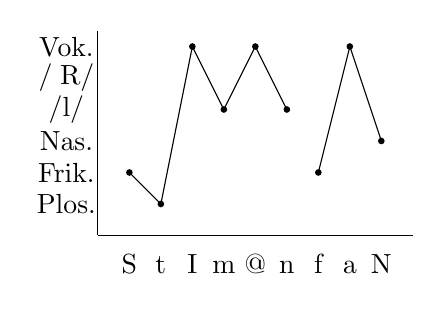
\begin{tikzpicture}[scale=0.4]
		\draw[black] (-1,0) -- (9,0) ; % x axis
		\draw[black] (-1,0) -- (-1,6.5); % y axis
		\node at (-2,1) {Plos.};
		\node at (-2,2) {Frik.};
		\node at (-2,3) {Nas.};
		\node at (-2,4) {\textipa{/l/}};
		\node at (-2,5) {\textipa{/\;R/}};
		\node at (-2,6) {Vok.};
		\draw[black] (0,2) -- (1,1) -- (2,6) -- (3,4) -- (4,6) -- (5,4);
		\draw[black] (6,2) -- (7,6) -- (8,3);
		\node at (0,-1) {\strut \textipa{S}};
		\node at (1,-1) {\strut \textipa{t}};
		\node at (2,-1) {\strut \textipa{I}};
		\node at (3,-1) {\strut \textipa{m}};
		\node at (4,-1) {\strut \textipa{@}};
		\node at (5,-1) {\strut \textipa{n}};
		\node at (6,-1) {\strut \textipa{f}};
		\node at (7,-1) {\strut \textipa{a}};
		\node at (8,-1) {\strut \textipa{N}};
		\fill (0,2) circle [radius=3pt];
		\fill (1,1) circle [radius=3pt];
		\fill (2,6) circle [radius=3pt];
		\fill (3,4) circle [radius=3pt];
		\fill (4,6) circle [radius=3pt];
		\fill (5,4) circle [radius=3pt];
		\fill (6,2) circle [radius=3pt];
		\fill (7,6) circle [radius=3pt];
		\fill (8,3) circle [radius=3pt];
	\end{tikzpicture}
\end{figure}

\end{columns}

\end{frame}


%%%%%%%%%%%%%%%%%%%%%%%%%%%%%%%%%%%%%%%%%%%%%%%
\begin{frame}{Hausaufgabe -- Lösung}


Zu (\ref{ex:03cHA1b})

\begin{columns}
	\column[b]{.5\textwidth}
	
\begin{figure}
\footnotesize
\centering
	\begin{forest} MyP edges, [, phantom
		[$\sigma$
		[O [x, tier=word [\textipa{m}]]] 
		[R [N [x, tier=word [\textipa{I}]]] [K [x, name=x1 [\textipa{t}]]]]
		]
		[$\sigma$
		[O, name=onset1]
		[R [N [x [\textipa{a:}, name=a]]
		[x, name=ax]] [K [x [\textipa{k}]]]]
		]
		[$\sigma$
		[O [x, tier=word [\textipa{P}]]]
		[R [N [x [\textipa{E}]]] [K [x, name=x2 [\textipa{s}]]]]
		]
		[$\sigma$
		[O, name=onset2]
		[R [N [x [\textipa{\textsyllabic{n}}]]]
		]
		]]
		{
		\draw[black] (x1.north)--(onset1.south);
		\draw[black] (x2.north)--(onset2.south);
		\draw[black] (a.north)--(ax.south);
		}
	\end{forest}
\end{figure}

\pause
\column[b]{.5\textwidth}

\begin{figure}
	\footnotesize
	\centering
	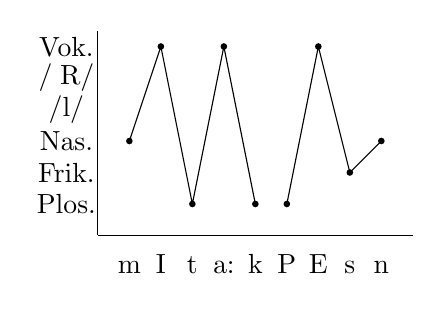
\begin{tikzpicture}[scale=0.4]
		\draw[black] (-1,0) -- (9,0) ; % x axis
		\draw[black] (-1,0) -- (-1,6.5); % y axis
		\node at (-2,1) {Plos.};
		\node at (-2,2) {Frik.};
		\node at (-2,3) {Nas.};
		\node at (-2,4) {\textipa{/l/}};
		\node at (-2,5) {\textipa{/\;R/}};
		\node at (-2,6) {Vok.};
		\draw[black] (0,3) -- (1,6) -- (2,1) -- (3,6) -- (4,1);
		\draw[black] (5,1) -- (6,6) -- (7,2) -- (8,3);
		\node at (0,-1) {\strut \textipa{m}};
		\node at (1,-1) {\strut \textipa{I}};
		\node at (2,-1) {\strut \textipa{t}};
		\node at (3,-1) {\strut \textipa{a:}};
		\node at (4,-1) {\strut \textipa{k}};
		\node at (5,-1) {\strut \textipa{P}};
		\node at (6,-1) {\strut \textipa{E}};
		\node at (7,-1) {\strut \textipa{s}};
		\node at (8,-1) {\strut \textipa{\textsyllabic{n}}};
		\fill (0,3) circle [radius=3pt];
		\fill (1,6) circle [radius=3pt];
		\fill (2,1) circle [radius=3pt];
		\fill (3,6) circle [radius=3pt];
		\fill (4,1) circle [radius=3pt];
		\fill (5,1) circle [radius=3pt];
		\fill (6,6) circle [radius=3pt];
		\fill (7,2) circle [radius=3pt];
		\fill (8,3) circle [radius=3pt];
	\end{tikzpicture}
\end{figure}

\end{columns}

\end{frame}


%%%%%%%%%%%%%%%%%%%%%%%%%%%%%%%%%%%%%%%%%%%%
\begin{frame}{Hausaufgabe -- Lösung}

Zu (\ref{ex:03cHA1b})  (alternative Lösung):

\begin{columns}
	\column[b]{.5\textwidth}
	
	
\begin{figure}
\footnotesize
\centering

	\begin{forest} MyP edges, [, phantom
		[$\sigma$
		[O [x, tier=word [\textipa{m}]]] 
		[R [N [x, tier=word [\textipa{I}]]] [K [x, name=x1 [\textipa{t}]]]]
		]
		[$\sigma$
		[O, name=onset1]
		[R [N [x [\textipa{a:}, name=a]]
		[x, name=ax]] [K [x [\textipa{k}]]]]
		]
		[$\sigma$
		[O [x, tier=word [\textipa{P}]]]
		[R [N [x [\textipa{E}]]] [K [x, name=x2 [\textipa{s}]]]]
		]
		[$\sigma$
		[O, name=onset2]
		[R [N [x [\textipa{@}]]] [K [x [\textipa{n}]]]]
		]
		]
		{
		\draw[black] (x1.north)--(onset1.south);
		\draw[black] (x2.north)--(onset2.south);
		\draw[black] (a.north)--(ax.south);
		}
	\end{forest}

\end{figure}

\pause

\column[b]{.5\textwidth}

\begin{figure}
\footnotesize
\centering
	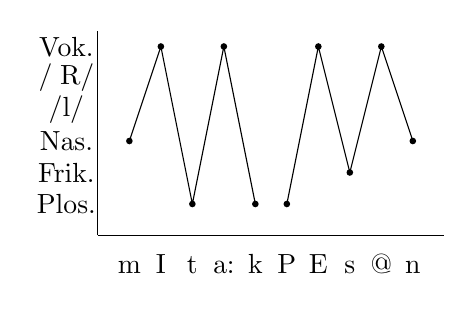
\begin{tikzpicture}[scale=0.4]
		\draw[black] (-1,0) -- (10,0) ; % x axis
		\draw[black] (-1,0) -- (-1,6.5); % y axis
		\node at (-2,1) {Plos.};
		\node at (-2,2) {Frik.};
		\node at (-2,3) {Nas.};
		\node at (-2,4) {\textipa{/l/}};
		\node at (-2,5) {\textipa{/\;R/}};
		\node at (-2,6) {Vok.};
		\draw[black] (0,3) -- (1,6) -- (2,1) -- (3,6) -- (4,1);
		\draw[black] (5,1) -- (6,6) -- (7,2) -- (8,6) -- (9,3);
		\node at (0,-1) {\strut \textipa{m}};
		\node at (1,-1) {\strut \textipa{I}};
		\node at (2,-1) {\strut \textipa{t}};
		\node at (3,-1) {\strut \textipa{a:}};
		\node at (4,-1) {\strut \textipa{k}};
		\node at (5,-1) {\strut \textipa{P}};
		\node at (6,-1) {\strut \textipa{E}};
		\node at (7,-1) {\strut \textipa{s}};
		\node at (8,-1) {\strut \textipa{@}};
		\node at (9,-1) {\strut \textipa{n}};
		\fill (0,3) circle [radius=3pt];
		\fill (1,6) circle [radius=3pt];
		\fill (2,1) circle [radius=3pt];
		\fill (3,6) circle [radius=3pt];
		\fill (4,1) circle [radius=3pt];
		\fill (5,1) circle [radius=3pt];
		\fill (6,6) circle [radius=3pt];
		\fill (7,2) circle [radius=3pt];
		\fill (8,6) circle [radius=3pt];
		\fill (9,3) circle [radius=3pt];
	\end{tikzpicture}
\end{figure}

\end{columns}

\end{frame}


%%%%%%%%%%%%%%%%%%%%%%%%%%%%%%%%%%%%%%%%%%%%%%%
\begin{frame}{Hausaufgabe -- Lösung}

Zu (\ref{ex:03cHA1c}):

\begin{columns}
	\column[b]{.5\textwidth}
	
\begin{figure}
\centering
	\begin{forest} MyP edges, [, phantom
		[$\sigma$
		[O [x,tier=word [\textipa{b}]]]
		[R [N [x, tier=word [\textipa{i:}, name=i]] [x,name=x1]] [K [x [\textipa{5}]]]]
		]
		[$\sigma$
		[O [x, tier=word [\textipa{d}]]]
		[R [N [x [\textipa{E}]]] [K [x, name=x [\textipa{k}]]]]
		]
		[$\sigma$
		[O, name=onset]
		[R [N [x, tier=word [\textipa{@}]]] [K [x [\textipa{l}]]]]
		]
		]
		{
		\draw[black] (x1.south)--(i.north);
		\draw[black] (x.north)--(onset.south);
		}
	\end{forest}
\end{figure}

\pause

\column[b]{.5\textwidth}

\begin{figure}
\centering
	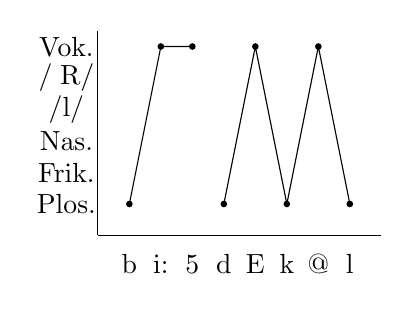
\begin{tikzpicture}[scale=0.4]
		\draw[black] (-1,0) -- (8,0) ; % x axis
		\draw[black] (-1,0) -- (-1,6.5); % y axis
		\node at (-2,1) {Plos.};
		\node at (-2,2) {Frik.};
		\node at (-2,3) {Nas.};
		\node at (-2,4) {\textipa{/l/}};
		\node at (-2,5) {\textipa{/\;R/}};
		\node at (-2,6) {Vok.};
		\draw[black] (0,1) -- (1,6) -- (2,6);
		\draw[black] (3,1) -- (4,6) -- (5,1) -- (6,6) -- (7,1);
		\node at (0,-1) {\strut \textipa{b}};
		\node at (1,-1) {\strut \textipa{i:}};
		\node at (2,-1) {\strut \textipa{5}};
		\node at (3,-1) {\strut \textipa{d}};
		\node at (4,-1) {\strut \textipa{E}};
		\node at (5,-1) {\strut \textipa{k}};
		\node at (6,-1) {\strut \textipa{@}};
		\node at (7,-1) {\strut \textipa{l}};
		\fill (0,1) circle [radius=3pt];
		\fill (1,6) circle [radius=3pt];
		\fill (2,6) circle [radius=3pt];
		\fill (3,1) circle [radius=3pt];
		\fill (4,6) circle [radius=3pt];
		\fill (5,1) circle [radius=3pt];
		\fill (6,6) circle [radius=3pt];
		\fill (7,1) circle [radius=3pt];
	\end{tikzpicture}
\end{figure}

\end{columns}

\end{frame}


%%%%%%%%%%%%%%%%%%%%%%%%%%%%%%%%%%%%%%%%%%%%%%%%%%%
\begin{frame}{Hausaufgabe -- Lösung}
\begin{itemize}
\item[2.] Silbifizieren Sie folgende Segmentsequenzen \textbf{in zwei Schritten}:
\begin{itemize}
\item Onsetmaximierungsprinzip
\item Sonoritätsprinzip
\end{itemize}

Stellen Sie fest, ob alle Silben wohlgeformt sind.\\
Falls nicht, benennen Sie die Verletzungen.

\begin{exe}
\exr{ex:03cHA2} Urinstinkt
\pause
\begin{xlist}
	\ex \alertred{\textipa{[Pu.\;RI.nStInkt]} (Onsetmaximierung)} \pause
	\ex  \alertred{\textipa{[Pu.\;RIn.(\,S\,)tInkt]} (Sonoritätsprinzip, \textipa{S} ist extrasilbisch)} \pause
	\ex  \alertred{\textipa{[Pu5.PIn.stinkt]} (Silbifizierung)}
\end{xlist}
\end{exe}
\pause

\item (\ref{ex:03cHA2}a) und (\ref{ex:03cHA2}b) sind einfach nach der Lautfolge silbifiziert.\\
Silbifizierung erfolgt jedoch auf der Ebene des phonologischen Wortes.\\
Daher werden die phonologischen Wörter \ab{ur-} und \ab{Instinkt} einzeln silbifiziert.
\end{itemize}
\end{frame}

%%%%%%%%%%%%%%%%%%%%%%%%%%%%%%%%%%%%%%%%%%%%%%%%

\begin{frame}{Hausaufgabe -- Lösung}
\begin{itemize}	
\item[3.] Geben Sie die standarddeutsche \textbf{phonetische Transkription} des Wortes \ab{Stahltische} inklusive der \textbf{Silbenstruktur} (mit X-Skelettschicht) an. Ermitteln Sie die \textbf{Kriterien}, die bei der Silbifizierung wirken.
\end{itemize}

\pause

\begin{minipage}{.5\textwidth}
\begin{figure}
\scalebox{.8}{\begin{forest}
MyP edges [, phantom
[$\sigma$
[O 
[x, tier=word[\textipa{S}]]
[x, tier=word[\textipa{t}]]
]
[R
[N
[x, tier=word[\textipa{a:}, name=a]]
[x, name=x]
]
[K[x[\textipa{l}]]]
]
]
[$\sigma$
[O [x, tier=word[\textipa{t}]]]
[R
[N
[x[\textipa{I}]]
]
[K
[x,name=S[\textipa{S}] ]
]
]
]
[$\sigma$
[O, name=o]
[R
[N
[x[\textipa{@}]]
]
]
]
]
\draw[black](o.south)--(S.north);
\draw[black](a.north)--(x.south);
\end{forest}}
\end{figure}
\end{minipage}
\begin{minipage}{.45\textwidth}
	
\pause	
	
\begin{itemize}
\item Onset-Maximierung \pause
\item Sonoritätshierarchie im Onset: *Sonorant vor Obstruent (*[\textipa{lt}]) \pause
\item Silbengelenk nach ungespanntem, betontem Vokal
\end{itemize}
\end{minipage}

\end{frame}

%%%%%%%%%%%%%%%%%%%%%%%%%%%%%%%%%%%%%

\begin{frame}{Hausaufgabe -- Lösung}
\begin{itemize}

\item[4.] Geben Sie die Gründe an, warum die folgenden Wörter aus phonetisch/""phonologischen Gründen im Deutschen nicht möglich sind:

\begin{exe}
	\exr{ex:03cHA3}
	\settowidth\jamwidth{XXXXXXXXXXXXXXXXXXXXXXXXXXXXXXXXXXX}
	\begin{xlist}
		\ex[*]{ \textipa{['Napl.O:t]}
			\loesung{2}{Onset-Maximierung \textipa{[pl]}, \textipa{[N]} steht am Wortanfang,} 
			\loesung{2}{\textipa{[O]} ist ungespannt und lang} }
		\ex[*]{ \textipa{[a\;R.'tUng]}
			\loesung{3}{Auslautverhärtung, regressive velare nasale Assimilation,}\loesung{3}{Knacklaut} }
	\end{xlist}

\end{exe}

\end{itemize}

\end{frame}


%% -*- coding:utf-8 -*-

%%%%%%%%%%%%%%%%%%%%%%%%%%%%%%%%%%%%%%%%%%%%%%%%%%%%%%%%%


\def\insertsectionhead{\refname}
\def\insertsubsectionhead{}

\huberlinjustbarfootline


\ifpdf
\else
\ifxetex
\else
\let\url=\burl
\fi
\fi
\begin{multicols}{2}
{\tiny
%\beamertemplatearticlebibitems

\bibliography{gkbib,bib-abbr,biblio}
\bibliographystyle{unified}
}
\end{multicols}





%% \section{Literatur}
%% \begin{frame}[allowframebreaks]
%% \frametitle{Literatur}
%% 	\footnotesize

%% \bibliographystyle{unified}

%% 	%German
%% %	\bibliographystyle{deChicagoMyP}

%% %	%English
%% %	\bibliographystyle{chicago} 

%% 	\bibliography{gkbib,bib-abbr,biblio}
	
%% \end{frame}



\end{document}